\documentclass[serif,aspectratio=169]{beamer}
\usepackage[normalem]{ulem}

\usepackage{../theme/flagbot}

% warns about obsolete commands
\usepackage{nag}

%% Font preferences
%\usepackage[oldstyle,semibold]{libertinus} % not good on black bg
\usepackage[oldstyle,semibold]{noto}

% self-explanatory
\usepackage{qrcode}

%\setbeameroption{show notes on second screen}

\tikzstyle{freecell}=[fill=none]

\newcommand{\reg}[1]{\%\mintinline{asm}{#1}}
\newcommand{\hex}[1]{\mintinline{python}{0x#1}}
\newcommand{\naddr}[2]{\begin{tabular}{l}#1\\\hex{#2}\end{tabular}}
\newcommand{\docl}[1]{(\textbf{\href{#1}{Documentation}})}


%% Proper 1337 typography
\newcommand\SlashedZero{{%
\addfontfeatures{RawFeature=+zero}%
\addfontfeatures{RawFeature=-pnum}%
\addfontfeatures{RawFeature=-onum}%
0%
}}
\newcommand\organizers{\SlashedZero{}rganizers}
\newcommand\polyglots{polygl\SlashedZero{}ts}

\newcommand\biglink[1]{
	\begin{center}
		\colorbox{white}{
		\textcolor{black}{
		\qrcode*[height=.8\textheight]{#1}
	}
	}

		\url{#1}
	\end{center}
}

\hypersetup{colorlinks,linkcolor=,urlcolor=brightblue}

\setbeamertemplate{navigation symbols}{}

\setbeameroption{show notes}

\showsectionframe{}

%%%%%%%%%%%%%%%%%%%%%%%%%%%%%%%%%%%%%%%%%%%%%%%%%%%%%%%%%%%%%%%%%%%%%%%%%%%%%%%
% Title Setup
%%%%%%%%%%%%%%%%%%%%%%%%%%%%%%%%%%%%%%%%%%%%%%%%%%%%%%%%%%%%%%%%%%%%%%%%%%%%%%%
\title{crypto survival guide}
\author{\texttt{lourkeur}}
\institute{\polyglots}
\date{\today}
\begin{document}
\titleframe{}
\note{
	name is Louis blahblahblah

	18 months ago I was sitting in the audience here trying to get into CTF\@.
	I also started an MSc to help with getting flags.
	Now I have this little guy in my discord nickname.
}

\begin{frame}
	\begin{center}
	
\includegraphics{psyduck.png}
	\end{center}
	\note{
		I am a crypto player in the number one CTF team in the world.
		That's what I call success!
		And I'm going to tell you how to get there for absolutely free.
	}
\end{frame}
\begin{frame}
	\frametitle{What is crypto?}
	\note{
		So first thing is what am I doing exactly?
		What is this crypto thing?

		So yeah it stands for cryptology and cryptography.
		We're not talking about the other ``cryptos''.
		There's like twenty thousand by now or something?
		Anyways.
	}
\end{frame}
\begin{frame}
	\frametitle{What is crypto?}
	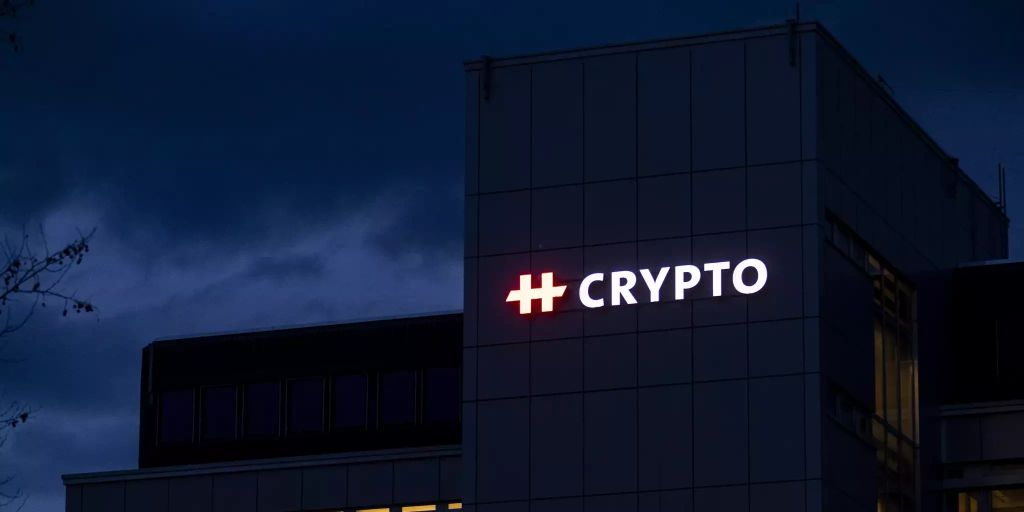
\includegraphics[width=\textwidth]{crypto-ag.jpg}
	\note{
		This type of crypto.
		Mathematical tools that people use to protect their flags.
	}
\end{frame}
\begin{frame}
	\frametitle{Which crypto?}
	\begin{itemize}
		\item Classical
		\item Modern
	\end{itemize}
	\note{
		So there are two categories of crypto.
		Classical is algorithms that could be used before computers were available,
		Modern is computer-assisted stuff.

		Right now the meta in CTFs leans more on modern crypto
		but we will also cover a bit of classical
	}
\end{frame}
\begin{frame}
	\frametitle{Prerequisites}
	\begin{itemize}
	\pause{}
\item discrete algebra
\item probability theory
	\pause{}
\item crypto basics
	\end{itemize}
	\note{
		one bad thing with the crypto category is it can be less approachable because of all the math.
		OTOH it's also an opportunity to learn!
		let's list them a bit.
		I'm not going to do a show of hands to avoid singling anyone out.
		You can think for yourself.

		Looking at algebra and probabilities I think most EPFL bachelor programs include those.
		Other tech universities are probably similar.
		Anyways, if you're not comfortable with some of those elements, ask around!

		for crypto basics there's Computer Security in the bachelor an minors program here.
		If you did well on that course you're going to do well. If not, I recommended a free talk by JP Aumasson in the announcements this week. so here's it again, don't hesitate to check it out.
	}
\end{frame}
\begin{frame}
	\frametitle{Introduction to Cryptography}
	\biglink{https://youtu.be/ah5rIeKDNsU}
\end{frame}
\begin{frame}
	\frametitle{How to approach a crypto chal}
	\note{
		let's look at how I approach a challenge.
	}
\end{frame}
\begin{frame}
	\frametitle{The CTF cheatsheet}
	\pause{}
	\begin{center}
		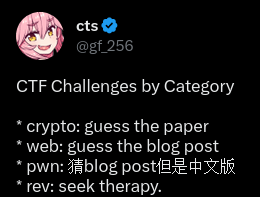
\includegraphics[height=0.8\textheight]{ctf_cheat_sheet.png}
	\end{center}
	\note{
		So the cheatsheet tells us to ``guess the paper''.
		There's a research paper out there that this chall is based on.
		How do we find papers?

		Second thing is knowing how to search.
		Most of the time there's something obscure for you to learn.
	}
\end{frame}
\begin{frame}
	\frametitle{Preprints}
	\begin{center}
		
\includegraphics[width=.4\textwidth]{iacrlogo.png}

	\url{https://eprint.iacr.org/}
	\end{center}
\end{frame}
\begin{frame}
	\frametitle{Preprints}
	\begin{center}
		
\includegraphics[width=.5\textwidth]{arxiv-logo.png}

		\url{https://arxiv.org/}
	\end{center}
	\note{
		There's a long tradition of Open Access in cryptology.
		This means that the vast majority of researchers will publish their papers online free-of-charge.
		(That's what makes it possible to do CTF at all)

		crypto eprints, specialized
		ArXiv, mathematics
	}
\end{frame}
\begin{frame}
	\frametitle{Abstraction levels}
	\emph{Program to an interface, not to an implementation}
	\note{
		Going back to levels of abstraction.
		There's a saying in software engineering.

		This is also the case in cryptography.

		Is the author re-implementing a primitive explicitly?
		Probably done on purpose.
		If they are using a well-known library then the issue is probably with interactions.

		For the longest time I thought elliptic curve formulas were confusing.
		Instead of bothering to study them more,
		I just took it for granted that they worked as an Abelian group and that the discrete logarithm was hard.
		And in a lot of cases that's all you need.
		Occasionally there are challs with broken elliptic curves or something,
		so I just left them for soemone else who's more advanced or more specialized.
	}
\end{frame}
\begin{frame}
	\frametitle{Tools of the trade: Cyberchef}
	\begin{center}
		\biglink{https://cyberchef.org/}
	\end{center}
	\note{
		First tool: cyberchef
		It's a toolbox that runs in your browser and can do various transformations on pieces of data.
		Let's check it out a bit.
		point out entropy, magic, modern ciphers, classical ciphers, filetype detection
		of course you can also do all of this on the terminal if you prefer
	}
\end{frame}
\begin{frame}
	\frametitle{Tools of the trade: Python 3}
Python has super\texttt{pow}ers
	\note{
		Python 3 is the most common language for both challs and solvescripts.
		The reason: with just the built-in stuff you already have modular exponentiation for arbitrarily big numbers
		Also the usual bitwise operations, standard hashes, etc.
		To prove this, here's a toy implementation of DSA signature generation.
	}
\end{frame}
\begin{frame}[fragile]
	\inputminted[]{python}{dsa_sign.py}
	\note{
		don't use this for serious stuff, it's just to show that it's here
		we're not done with python: let's talk about the libraries
	}
\end{frame}
\begin{frame}
	\frametitle{Tools of the trade: Python libs}
	\begin{itemize}
\item \texttt{pwntools}
\item \texttt{PyCryptoDome}
\item \texttt{fastecdsa}
\item Extra stuff from PyPI\@: \texttt{passlib}, \texttt{pgpy}, \texttt{blspy}, \texttt{web3} etc.
	\end{itemize}

	\note{

		You will want pwntools to talk with any remotes.
		You already know it, no need to look any further.

		PyCryptoDome has a lot of low-level crypto primitive and serialization formats.
		Get it too, it's free!

		If you need elliptic curve math, fastecdsa is your friend

		And if you need to go beyond that, PyPI has almost everything so search
	}


\end{frame}
\begin{frame}
	\frametitle{Polygl0ts docker}
	\begin{center}
		\biglink{https://ghcr.io/polygl0ts/crypto.docker}
		\note{we have a docker set up with some common libraries here if you'd like. It has jupyter in it}
	\end{center}
\end{frame}
\begin{frame}
	\frametitle{Tools of the trade: Sage}
	\note{
		The last tool is SageMath. It's a sofware system for mathematicians.
		In more esoterc challenges you might encounter it.

		There's this language that's overlaid on top of Python 3 but it's different in subtle ways
		I personally don't really like it because there are a lot of weird footguns lying around but you might still need it.
	}
\end{frame}
\begin{frame}
	\frametitle{Cryptohack docker}
	\begin{center}

		\biglink{https://github.com/cryptohack/cryptohack-docker}
	\end{center}
	\note{This is the CryptoHack docker container which has sage in it and heavily inspired ours.}
\end{frame}
\begin{frame}
	\begin{itemize}
		\item play
		\item read writeups
		\item follow crypto stuff
	\end{itemize}
	\note{
		play CTFs with us, play cryptohack, play imaginary.
		Then read writeups.
		Other thing you can do is join cryptography communities on your favorite social media.
		You can get exposed to interesting stuff. And a lot of drama. With a side order of interesting stuff.
	}
\end{frame}
\begin{frame}
	\frametitle{GIVE ME FLAGS}
	\begin{center}
	\biglink{https://friday.polygl0ts.ch/}
	\end{center}
	\note{
		I know I'm boring and some of you have been listening to boring nerds talk about crypto for way too long, so it's time to roll
	}

\end{frame}
\end{document}
